%\documentstyle[twocolumn]{article}
%\documentclass[twocolumn,showpacs,showkeys,fleqn,prb]{revtex4}% Physical Review B
\documentclass[twocolumn,showpacs,showkeys,fleqn,prl,superscriptaddress]{revtex4}% Physical Review Letter
%\documentclass[preprint,showpacs,showkeys,fleqn,prb,superscriptaddress]{revtex4}% Physical Review B
%\documentclass[twocolumn,showpacs,showkeys,fleqn,prb,superscriptaddress]{revtex4}% Physical Review B
\usepackage{graphicx}% Include figure files
\usepackage{epstopdf}% eps <-> pdf 
\usepackage{dcolumn}% Align table columns on decimal point
\usepackage{bm}% bold math
\usepackage{amssymb}
\usepackage{amsmath} 
\usepackage{xcolor}
%\usepackage{multicol}
%\usepackage{umlaut}
\newcommand{\bb}[1]{\textbf{ #1}}
\newcommand{\nn}[1]{\textnormal{ #1}}
\newcommand{\ii}[1]{\textit{#1}}
\newcommand{\fs}[1]{\footnotesize{#1}}
\newcommand{\ns}[1]{\normalsize{#1}}

\newcommand{\bra}[1]{\langle #1|}
\newcommand{\ket}[1]{|#1\rangle}
\newcommand{\braket}[2]{\langle #1|#2\rangle}

\newcommand{\ini}{\nn{\!i}}
\newcommand{\fin}{\nn{\!f}}
\newcommand{\iqr}{i\!\bb{Q}\cdot\!\!\bb{r}} 
\newcommand{\eiqr}{e^{i\!\bb{Q}\cdot\!\bb{r}}} 
\newcommand{\aii}{\nn{\!\!I\!I}} 
\newcommand{\aiii}{\nn{\!\!I\!I\!I}} 

\begin{document}
%\preprint{et al.}

\title{
Direct observation of momentum distribution and renormalization factor in lithium
}

\author{ 
N.~Hiraoka
}
\email{hiraoka@spring8.or.jp}
\affiliation{
National Synchrotron Radiation Research Center,
Hsinchu, 30076, Taiwan
}

\author{ 
K.~Matsuda
}
\affiliation{
Graduate School of Science, Kyoto University, Kyoto 606-8502, Japan
}

\author{ 
T.~Hagiya
}
\affiliation{
Graduate School of Science, Kyoto University, Kyoto 606-8502, Japan
}
  
\author{ 
A.~Niozu
}
\affiliation{
Graduate School of Science, Kyoto University, Kyoto 606-8502, Japan
}


\author{ 
S.~Huotari
}
\affiliation{
Department of Physics, POB 64, FI-00014, University of Helsinki, Helsinki, Finland
}

\author{ 
Y.~Yang
}
\affiliation{
Department of Physics, University of Illinois, Urbana, Illinois 61801, USA
}

\author{ 
M.~Holzmann
}
\affiliation{
LPTMC, Universite Pierre et Marie Curie and CNRS, 75005 Paris,
}

\author{ 
D.~M.~Ceperley
}
\affiliation{
Department of Physics, University of Illinois, Urbana, Illinois 61801, USA
}







\date{}
\begin{abstract}

An ultimate goal for electron momentum density measurements over their long history is to directly observe the momentum distribution of quasi particles in metals and determine the renormalization factor ${\color{violet}Z_{k_F}}$.
We have measured the momentum distribution in liquid and solid lithium by high-resolution Compton scattering so as to determine ${\color{violet}Z_{k_F}}$s.
High-resolution data over a wide momentum range exhibits a clear feature of the renormalization and a sharp drop of momentum densities at Fermi momentum $k_F$.
They are compared with those by ${\color{violet}Z_{k_F}}$ Monte Carlo simulation performed on a disordered crystal or glass, exhibiting very good agreement.        
Theoretical momentum distribution displays asymptotic behaviors as $(k/k_F)^4$ and $(k/k_F)^{-4}$ below and above $k_F$, respectively.
On the other hand, the experiment shows slightly smaller exponents. 
The experimentally and theoretically determined ${\color{violet}Z_{k_F}}$’s indicate a fairly good agreement with each other.


\end{abstract}
\pacs{78.70.Ck, 78.20.Ls}
% 78.70.Ck : x-ray scattering
% 78.20.Ls : magneto-optical effects
%\keywords{}
\maketitle



The behavior of correlated electrons is a general problem in condensed matter physics.
The non-interacting homogeneous electron gas (HEG) has an occupation number of 1 or 0 per spin and the boundary defines the Fermi surface. 
The interacting HEG has the occupation of decimal numbers because some portions of the densities are scattered out of the Fermi surfaces due to the electron correlation. Thus, the discontinuity of the occupation number is reduced but still partly survives on Fermi surfaces. This is a typical momentum distribution of quasi particles in metals and the remaining discontinuity represents the renormalization factor ${\color{violet}Z_{k_F}}$. 
This is a general concept comprising even strongly correlated electron systems such as heavy fermions.         
Nonetheless, there is virtually no opportunity to directly see such a momentum distribution in experiments.

An energy spectrum of Compton scattered photons provides information of electron momentum densities (EMDs) in a sample\cite{sch}.
Under the impulse approximation (IA)\cite{eisen70,kaplan03}, the differential scattering cross-section is proportional to the Compton profile (CP), which is defined as
\begin{equation}
\frac{d^2\sigma}{d\Omega dE} \,\propto \, J(p_z) = \int \!\! \int n(k_x,k_y,k_z\!=\!p_z) \;dk_x dk_y .
\end{equation}
Because of the energy and momentum conservation, $p_z$ and the scattered photon energy $E$ are transformable to one another once the incident photon energy $E_o$ and the scattering angle $\theta$ are given.  
In order to retrieve momentum density $n(\!\!\bb{k})$, a tomographic reconstruction is necessary from CPs measured along various directions.
For an isotropic sample, $n(\!\!\bb{k})$ can be obtained from the derivative of a single CP. 
\begin{equation}
n(k) = - \frac{1}{2 \pi p} \frac{d J(p)}{d p}  | _{p=k}   .
\end{equation}
Note that $n(k)$ {\color{violet}obtained in this way}  tends to diverge as $k$ $\to$ 0, often limiting the field of view.  
The advantage of Compton scattering is that a sum rule is available so that CP can be normalized by electron numbers in an atom or a certain unit, facilitating quantitative comparisons with theory and experiment on an absolute scale.
Though the observation of $n(k)$ and ${\color{violet}Z_{k_F}}$ is quite straightforward in principle, reports of direct observation are extremely rare because the resolution of the experiments is not {\color{violet}high} enough in many cases.
To our knowledge, a report on Na a decade ago is the only successful example\cite{simo10}.
Even in this case, $n(p)$ is only shown in a limited region near $k_F$, prohibiting a review the overall shape of $n(p)$.


\begin{figure}
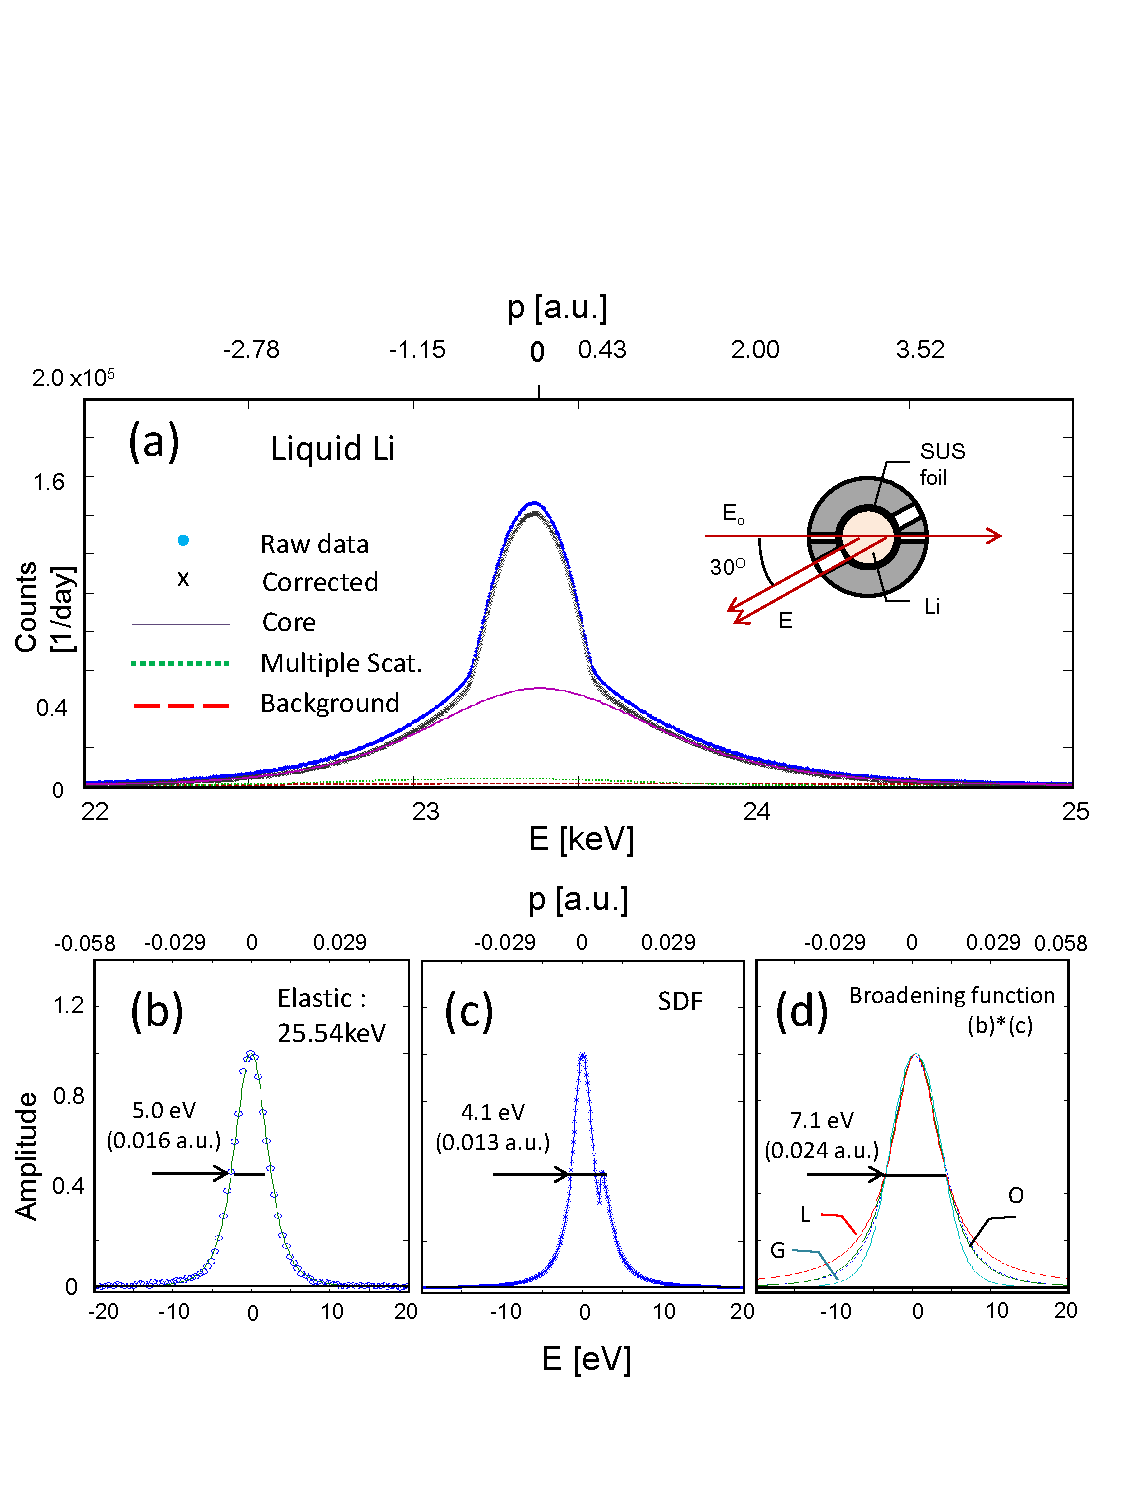
\includegraphics[bb= 30 50 500 600, width=7.5cm]{fig1.pdf}
\caption{(a) CPs for liquid Li: Inset shows geometry of the experiment. (b) Elastic line, monitoring the instrumental resolution, 
(c) Spectral density function, indicating the final-state broadening, (d) The convolution of \small{(b)} and (c), providing the broadening function for a comparison with theory. O is the optimally fitted function while G and L means Gaussian and Lorentzian, respectively.  
} 
\label{Fig.1}
\end{figure}



Na has free electrons showing isotropic nature and properties the closest to those of HEG among elementary metals.
Similarly, Li has also been investigated as a case in which the HEG model is applicable.
However, there is an unsolved puzzle standing for several decades for Li. 
Interacting HEG models generally predicate ${\color{violet}Z_{k_F}}$ of 0.6-0.7 for r$_s$=3.25 (Li).
The first experimental determination performed by Sch{\"u}lke \ii{et al.}\,provided 0.1$\pm$0.1 (along [100] axis) based on a model analysis on $n(p)$ obtained \ii{via} a reconstruction on a single crystal\cite{schulke96}. 
In fact, there was a common tendency upon comparisons between theories and experiments in past decades (still true at present) that theory generally predicted higher CPs in $p<p_F$ while lower in $p>p_F$\cite{saku95}. 
Kubo ascribed this to the electron correlation effects, showing that his GW calculation displayed a good agreement with experiments and indicating the substantially reduced ${\color{violet}Z_{k_F}}$ varying in 0.15-0.35 along several crystallographic axes\cite{kubo95,kubo97}.
Filippi and Ceperley elucidated CPs with {\color{violet}electron} correlation effect properly treated by ${\color{violet}Z_{k_F}}$ Monte Carlo (QMC) simulation, finally concluding that the correlation effect only partly accounted for the difference between theory and experiment, and claiming the necessity of other reasons\cite{filippi99}.  
Disorder effect\cite{dugdale98} and temperature effect on Li\cite{stern01} were discussed but they were not conclusive, leaving the puzzle unsolved.
Recently Klevak \ii{et al.}\,calculated EMD by real-space multiple-scattering Green-function approach and displayed a smooth drop of $n(k)$ at $k_F$ with an indiscernible ${\color{violet}Z_{k_F}}$ due to the disorder effect, rather resembling the curves by Kubo\cite{klevak16}.  
The source of the puzzle is that the conduction electrons in Li have a strong orbital hybridization with core electrons, leading to a large electron-lattice interaction.
This renders Fermi surface anisotropic and generates secondary Fermi surfaces in higher Brillouin zones due to Umklapp process.
They make quantitative comparisons between theory and experiment cumbersome. 

In this study, we have attempted a quantitative determination of ${\color{violet}Z_{k_F}}$ in Li by ultra-high resolution Compton scattering, where a 0.016 atomic unit (a.u.) instrumental resolution and a 0.024 a.u.\;overall resolution were achieved.
Solid Li has an anisotropic Fermi surface, posting the necessity of the EMD reconstruction for the exact evaluation. 
However, the reconstruction generally produces artifacts during complicated computing, making a quantitative analysis difficult.
We have measured liquid Li above the melting point.
The liquid sample can be considered perfectly isotropic, allowing us a straightforward derivation of $n(k)$ with minimized artifacts.
As a reference, we also measured a polycrystalline sample before melting the sample.
Both samples exhibit a clear break of $n(k)$ at $k_F$ and features of the renormalization, nicely showcasing the behaviors of the interacting HEG\cite{holz11}.

\begin{figure}
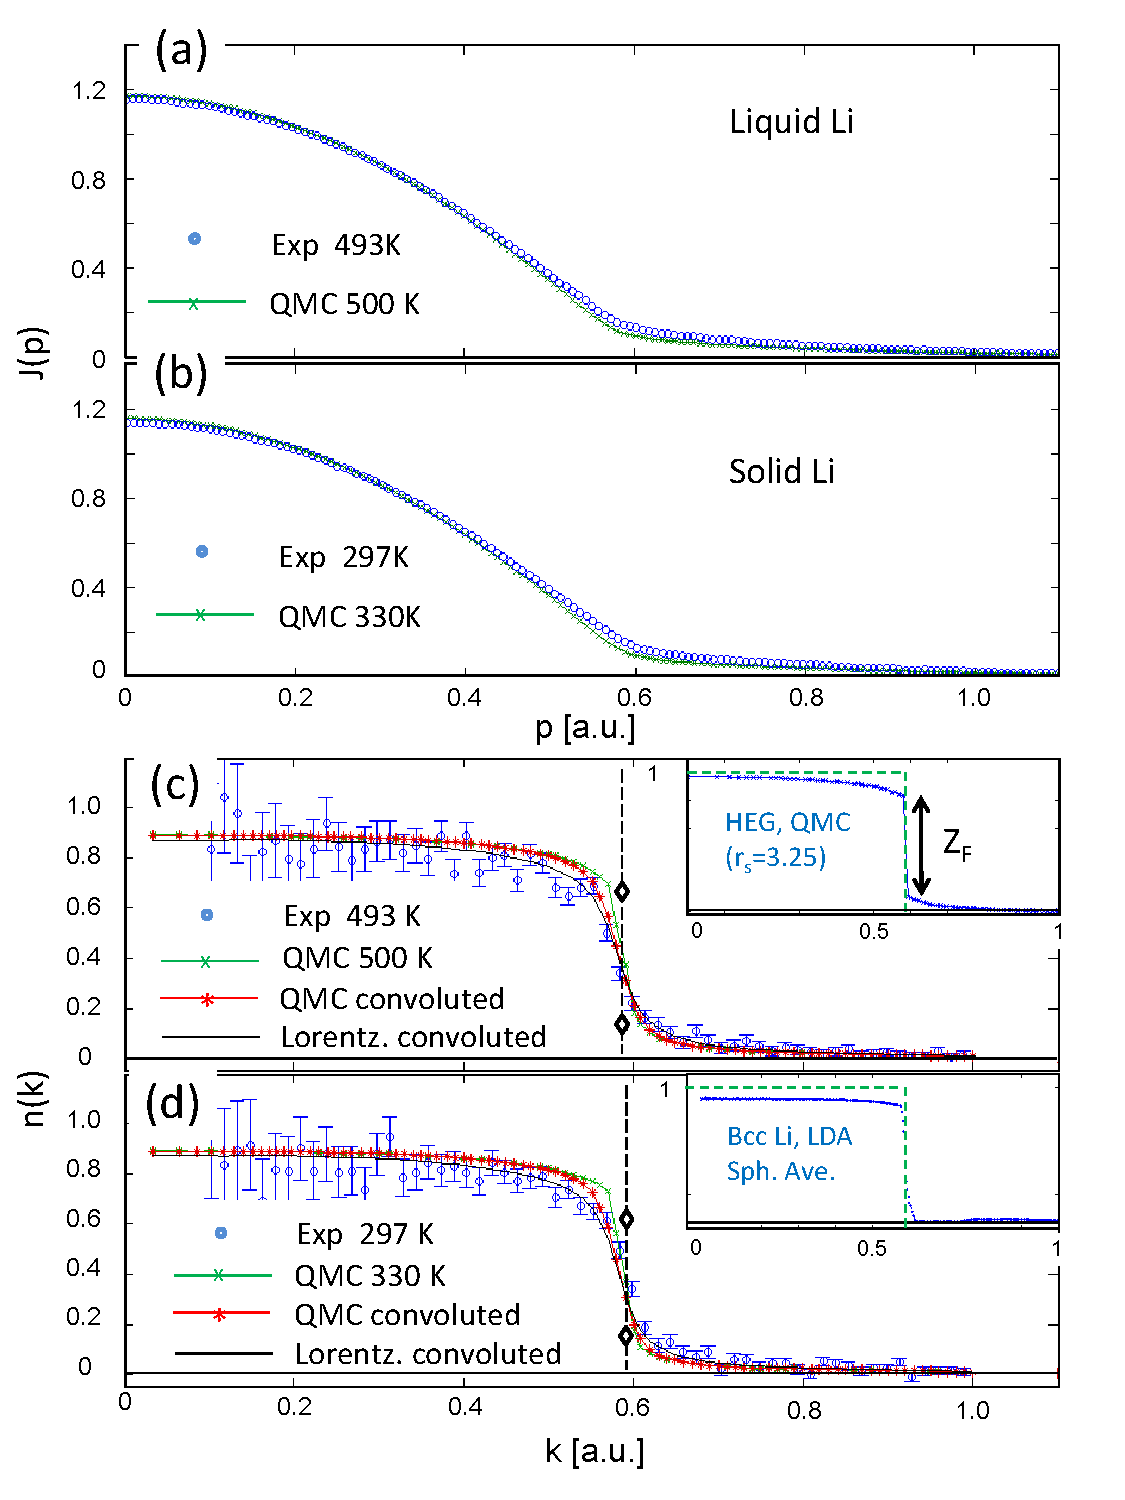
\includegraphics[bb= 50 10 500 720, width=7.5cm]{fig2.pdf}
\caption{CPs of liquid Li (a) and of solid Li (b), compared with theory convoluted by the broadening function, and EMDs in liquid (c) and solid Li (d), compared to theory with or without the convolutions. Inset shows spherical averaged EMD by band theory (LDA).  
} 
\label{Fig.2}
\end{figure}

The experiment was performed at Taiwan IXS beamline at SPring-8 (BL12XU).
The most critical parameter to determine ${\color{violet}Z_{k_F}}$ is the momentum resolution. 
A typical radius of a Fermi sphere is 0.5 - 1.0\,a.u. This fact requires a resolution of an order of 0.01\,a.u.\,to reveal ${\color{violet}Z_{k_F}}$, which is a technical challenge.
One can easily improve the instrumental resolution if low energy photons are used but the spectrum is substantially broadened by final-state effect\cite{stern00,soi01}.
We have chosen $E_o$=25.5 keV to obtain $dE$=5 eV (instrumental), corresponding to $dp$=0.016 a.u.
The details of the spectrometer are described in [\onlinecite{hira13}]. 


A polycrystalline Li sample having a cylindrical shape of 9-mm diameter and 10-mm height was placed in the furnace made of stainless steel (SUS) equipped with a heater at the bottom (Fig.1a inset).
The experiment was first performed at 297 K on solid Li and then at 493 K on liquid Li. 
The furnace had openings along the directions of incident photons and scattered photons (see, Fig.1a, inset).
The Li cylinder was rolled by a 10-$\mu$m thick SUS foil in a glovebox before setting, to avoid the sample spilling out of the furnace when Li was melt.
As seen in the figure, the scattered photons from the foil were blocked by the thick part of the furnace so that they were not detected.
The obtained CPs were corrected for the self-absorption, background, multiple scattering, and the energy dependence of the detection system (Fig.1a).


\vspace{10mm}

${\color{violet}Z_{k_F}}$ Monte Carlo calculations were performed on molecular dynamics (MD) configurations sampled at 330K and 500K for the solid and the liquid phases, respectively. The classical MD temperatures were elevated to roughly account for ${\color{violet}Z_{k_F}}$ fluctuations of the nuclei~\cite{filippi98}. We used Slater-Jastrow wavefunction with LDA orbitals on simulation cells containing 432 lithium atoms. Finite-size error of spherically average momentum distribution was corrected following~\cite{holz09}. Pseudopotential error was corrected using an all-electron calculation performed on the perfect crystal. All calculations were performed at the same density $r_s=3.25$. We rescaled the momentum distributions to experimental densities ($r_s=3.265$ for the solid and $r_s=3.31$ for the liquid) in post-processing. Fermi momenta of the MD configurations were determined by unfolding the LDA bands from 432-atom supercell to the primitive cell Brillouin zone. The unfolding has been performed using the BandUP code~\cite{Medeiros2014,Medeiros2015}.  We use LAMMPS~\cite{Plimpton1993} for the MD simulations, QE~\cite{Giannozzi2009,Enkovaara2017} for the DFT calculations, and QMCPACK~\cite{Kim2018} for the QMC calculations. The disordered calculations have been automated using the nexus suite of tools~\cite{Krogel2016}.
More computational details will be described elsewhere.

\vspace{10mm}





\begin{table}[b]
\begin{tabular}{llllllll}
\multicolumn{2}{l} {Averaging}   &      & $~n^+~~~$   & $~~n^-~~~$    & $~{\color{violet}\zeta_{k_F}}~~~$   & ~$n_o$~~~ & ${\color{violet}Z_{k_F}}$~   \\ \hline
 %            &    k range     & [au] &\footnotesize{0.50-0.55} & \footnotesize{0.63-0.68} &   &   &   \\ \hline
              & Theo. &\footnotesize{I}  & 0.80 & 0.046 & 0.76 & 0.89 & 0.82 \\ 
Liquid    &      &\footnotesize{II} & 0.77 & 0.052 & 0.71 & 0.89 & 0.78 \\
              &      &\footnotesize{III}& 0.70 & 0.074 & 0.62 & 0.87 & 0.70 \\ % \hline
              & Exp.  &      & 0.70 & 0.098 & 0.60 & 0.86 & 0.68 \\ \hline
                            & Theo. &\footnotesize{I}~~~~  & 0.81~~~ & 0.042~~~ & 0.77~~~ & 0.89~~~ & 0.84~~~ \\ 
Solid      &           &\footnotesize{II} & 0.78 & 0.045 & 0.74 & 0.89 & 0.80 \\
              &           &\footnotesize{III} & 0.71 & 0.067 & 0.64 & 0.87 & 0.72 \\ %\hline
              & Exp.  &      & 0.71 & 0.099 & 0.61 & 0.85 & 0.70 \\ \hline

\\
\multicolumn{2}{l} {Extrapolation}    &  &      &       &      &      &      \\ \hline
              & Theo. &\footnotesize{I} & 0.76 & 0.082 & 0.68 & 0.89 & 0.74 \\ 
Liquid    &      &\footnotesize{II}& 0.74 & 0.082 & 0.66 & 0.89 & 0.73 \\
              &     &\footnotesize{III} & 0.67 & 0.111 & 0.56 & 0.86 & 0.63 \\ % \hline
              & Exp.  &      & 0.69 & 0.142 & 0.54 & 0.86 & 0.62 \\ \hline
                  & Theo. &\footnotesize{I}  & 0.78 & 0.072 & 0.71 & 0.89 & 0.77 \\ 
Solid      &      &\footnotesize{II} & 0.76 & 0.074 & 0.69 & 0.89 & 0.75 \\
              &      &\footnotesize{II} & 0.69 & 0.104 & 0.58 & 0.87 & 0.65 \\ % \hline
              & Exp.  &      & 0.72 & 0.144 & 0.57 & 0.85 & 0.65 \\ \hline

\end{tabular}
\caption{ \label{tab:zkf}
${\color{violet}Z_{k_F}}$ and related parameters: ''Averaging'' means numbers obtained from $n(k)$ averaged around $k_F+\delta k$ or $k_F-\delta k$, where $\delta k$ is set 0.03 a.u.$\,$within a window of $\pm$0.025 a.u.
''Extrapolation'' means the numbers at $k \to k_F$ by linear fit in log-log scales.
Theory I.\, means from original QMC outputs, II.\,from those with the convolution, and III.\,from those with convolution by Lorentzian having long tails.
$n_o^{\nn{HEG}}$ = 0.97 is used.
} 
\end{table}


\begin{figure}
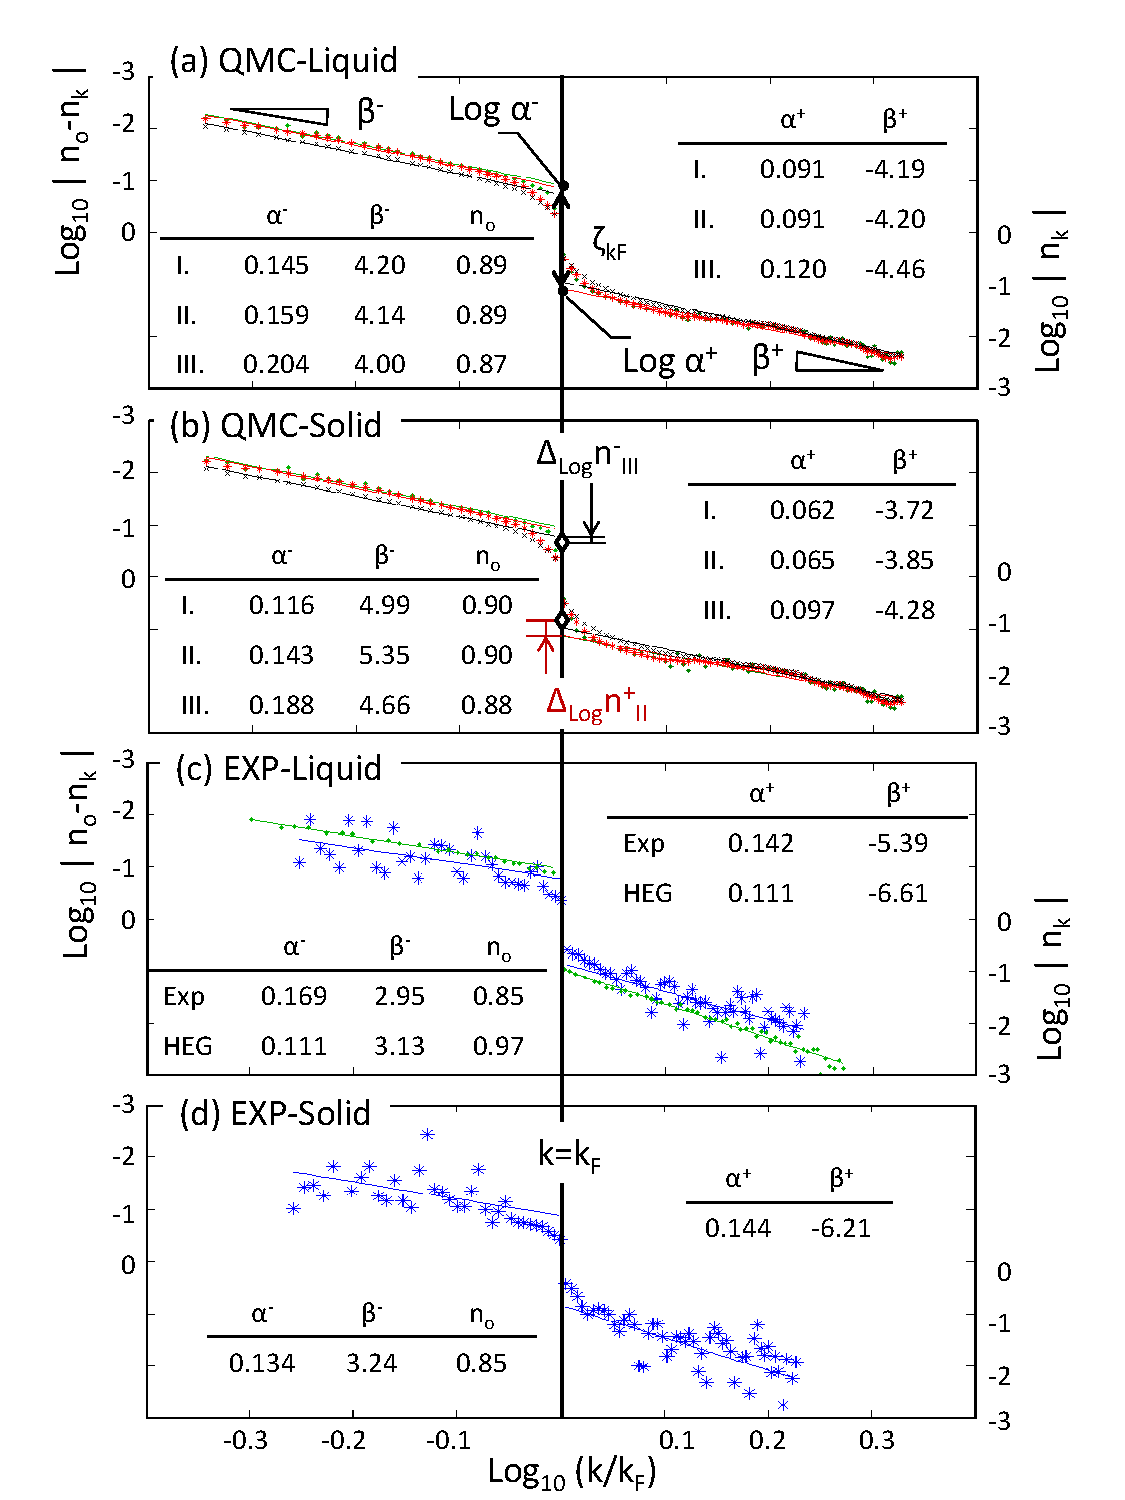
\includegraphics[bb= 70 10 500 700, width=7.5cm]{fig3.pdf}
\caption{Momentum densities plotted in the log-log scale:  Theories for liquid (a) andsolid (b), in which  [$\cdot$] indicates original outputs / Theory-I, [$*$] convoluted / Theory-II, and [$\times$] convoluted with Lorentzian / Theory-III.  Experiments on liquid (c) and solid (d).
} 
\label{Fig.3}
\end{figure}


Finally, theoretical CPs were convoluted by the broadening function due to the instrumental resolution and the final-state effect. 
The former was monitored by a line profile of the elastic scattering (Fig.1b), which had a width of 0.016 a.u.
For the latter, we calculated a spectral density function (SDF) for HEG based on Soininnen's form\cite{soi01}, which had a width of $\sim$ 0.013 a.u.\,(Fig.1c).
%The broadening function given by a sum of those functions showed a shape between Gaussian and Lorentzian.    
The broadening function given by a {\color{red}convolution} of those functions showed a shape between Gaussian and Lorentzian.
We fit this profile with an function $b(p) =1/ [ \Sigma_{n=0}^{n<3}\,a_n\,(2p / \Gamma )^{2n} ]$ and obtained ($a_0$, $a_1$, $a_2$) =(1.0, 0.85, 0.15) with $\Gamma$ = 0.024\,a.u.\,(Fig.1d).
Note this function becomes Lorentzian when (1, 1, 0) while nearly Gaussian when (0.6, 0.3, 0.1) as Taylor series. 

Figure 2a compares experimental valence CPs, $J(p)$ to theory (convoluted) while Fig.2b experimental EMDs $n(k)$’s to theory with and without convolutions. 
As a reference, one convoluted by Lorentzian having longer tails is also shown. 
The convolution was made in such a way that $J(p)$’s were first computed by Eq.(1), then convoluted, finally transformed back to $n(k)$’s by Eq. (2). 
EMDs of the liquid and solid Li are similar and clear features of the momentum distribution renormalization are recognized.  
Theory may be reproducing the experiment better when the Lorentzian-type broadening function is applied, in terms of the height of $n(k)$ and the curvatures near $k_F$, perhaps implying that SDF could have a larger tail than expected.
This possibility will be discussed later. 
Liquid Li has a slightly smaller density, and thus a smaller $k_F$, making $J(p)$ higher in $k < k_F$.
Furthermore, $n(k)$ in liquid shows slightly smoother drop at $ k_F $ due to a higher disorder effect and also to a larger correlation effect in the expanded system.
As mentioned above, solid Li has anisotropic Fermi surface and the radius of Fermi sphere varies in several \%\cite{saku95,schulke96}, This fact warns us of an easy comparison.
Nonetheless, those behaviors are quite consistent to what are expected across the melting point, indicating the solid sample consists of domains randomly oriented. 
A sharp drop at $k_F$ could remain even after the spherical averaging, as indeed examined on EMDs by band theory based on the local density approximation, (see, Inset in Fig.2d). 


First, we determine ${\color{violet}Z_{k_F}}$ as in the earlier report on Na\cite{simo10}, in which ${\color{violet}Z_{k_F}}$ is determined by the difference between $dJ/dp$ at $p\,$s slightly smaller and larger than $p_F$. 
This is equivalent to evaluating the difference between $n(k)$ at $k\,$s slightly smaller and larger than $k_F$.
Once one has $n^+$ and $n^-$ by averaging $n(k)$\,s among several points near $k_F-\delta k$ and  $k_F+\delta k$, respectively, the difference ${\color{violet}\zeta_{k_F}}$ = $n^+ - n^-$ provides the gap. 
Note that this is a renormalization factor that is reduced due to electron-lattice interaction. 
%The true ${\color{violet}Z_{k_F}}$ is obtained from ${\color{violet}\zeta_{k_F}}$$(n_o\,^{\nn{HEG}}/n_o) $.\footnote{this ratio is double-checked by LDA band-theory, where $n_o$=0.91 for bcc Li while it should be 1 without crystal potential.}  
${\color{violet}\zeta_{k_F}}{\color{red}(n_{k_F}^{\nn{FFG}}/n_{k_F}^{\nn{DFT}})}$.\footnote{this ratio is double-checked by LDA band-theory, where {\color{red}$n_{k_F}$=0.83} for bcc Li while it should be 1 without crystal potential.}
%Here, $n_o$ is experimental and theoretical $n(k)$ at $k \to 0$ obtained by an extrapolation while $n_o^{\nn{HEG}}$ that in HEG (=0.97). 
Here, $n_{k_F}^{\nn{FFG}}=1$ is the free Fermi gas (FFG) momentum distribution just inside the Fermi surface, while $n_{k_F}^{\nn{DFT}}$ is the DFT value, which accounts for electron-lattice interaction. 
The obtained ${\color{violet}Z_{k_F}}\,$s are summarized in the ``Averaging'' section of TABLE~\ref{tab:zkf}.



The advantage of the analysis above is {\color{violet}that it is} independent of the model but it obviously tends to overestimate ${\color{violet}Z_{k_F}}$s as the densities are read away from $k_F$.
According to the definition, ${\color{violet}Z_{k_F}}$ needs to be determined at the limit of $k$ $\to$ $k_F$. 
Sch{\"u}lke \ii{et al.}\,\,constructed a model where $n(k)$ decreases as $-(k/k_F)^{8}$ or $(k/k_F)^{-8}$ with increasing $k$\cite{schulke96}.
Based on their model, we first tried to plot $n(k)$ $vs$ $(k/k_F)^{\pm 8}$ but did not find a good linearity (not shown).
This fact encourages us to carefully investigate the asymptotic behaviors upon a more general model as follows: 
\begin{eqnarray}
n(k) &=& n_0 - \alpha^{+}  (k/k_F)^{\beta^+}  \;\;\;\; (k \leq k_F)  \nonumber \\
&=&  \alpha^{-}  (k/k_F)^{\beta^-}  \;\;\;\;\;\;\;\;\;\;\;\; (k>k_F)
\end{eqnarray}
Here, $\alpha^{+(-)}$ indicate the densities extrapolated at ${k=0\,(\infty) \to k_F}$ and $\beta^{+(-)}$ the exponent.
The $+$ (or $-$) sign represents the extrapolation along the positive (negative) direction on $k$ axis.

Figure 3 shows the log-log plots for $n(k)$ vs $(k/k_F)$, on which linear fits are indicated together. 
Theoretical $n(k)$ has the exponents $\beta$$\sim\pm$4, depending on the broadening functions.
HEG system would have $\beta$ = -8 at $k \gg k_F$, which is very different from the present one.
The reasons for the difference is (i) that HEG can have a different behavior as $k$ approaches $k_F$ and (ii) that Umklapp feature may significantly influence the asymptotic behaviors.
The experiments, on the other hand, shows $\beta^+$$\sim\,$3 and $\beta^-$$\sim\,$5. 
The non-negligible difference between theory and experiment may be due to Umklapp features that appear more prominent in theory.
It is noted that, if the average was taken for the absolutes $| \beta^+ |$ and $| \beta^- |$, it would be 4$\sim$5, which agrees with theory.
This exponent may be a characteristic parameter describing behaviors in a practical $k$ range.
Now we determine ${\color{violet}Z_{k_F}}$s. 
The extrapolated densities $\alpha^+$ and $\alpha^-$ give $n_o - n^+$ and $n^-$, respectively.
As mentioned already,  and ${\color{violet}Z_{k_F}}$ is given by ${\color{violet}\zeta_{k_F}}{\color{red}(n_{k_F}^{\nn{FFG}}/n_{k_F}^{\nn{DFT}})}$, where ${\color{violet}\zeta_{k_F}}= n^+ - n^-$.   
TABLE~\ref{tab:zkf} summarizes the ${\color{violet}Z_{k_F}}$s. 
The theory originally provides $Z_F$ = 0.76 for liquid and 0.78 solid  (see, Theory-I in TABLE~\ref{tab:zkf}) .
They are diminished to 0.74 and 0.76 after the convolution by $b(p)$ (Theory-II), meaning the experimentally observed $Z_F$ requires the correction for this, which amounts to 2.8 \%.
The experimental $Z_F\,$s are 0.62 (L) and 0.65 (S). After the corrections, we have $Z_F\,$s = 0.64 (L) and 0.67 (S) at the end.    


\vspace{10mm}

The log-log fits still tend to overestimate $Z_{k_F}$ because the momentum distribution is expected to have divergent slope at $k_F$~\cite{gg02}. To overcome this bias, we fit the QMC $n(k)$ to exact RPA form in a small region around $k_F$. Specifically, the QMC momentum distribution of each MD configuration is scaled to the range $\tilde{n}(x) \in [0, 1]$, where $x\equiv k/k_F$. Then, data near the Fermi break $x\in(0.8, 0.97)$ and $x\in(1.02, 1.2)$ are separately fitted to eq.~(\ref{eq:rpa-nk})
\begin{equation} \label{eq:rpa-nk}
\tilde{n}(x) = n_1 + A\vert 1-x\vert log\left(\vert 1-x\vert\right),
\end{equation}
where $n_1$ and $A$ are fitting parameters. Points too close to the $k_F$ are excluded because spherical average of anisotropic $n(\boldsymbol{k})$ smears out the Fermi break. The $n(k)$ discontinuity is extracted as the difference between the $n_1$ parameter of the left and right fits $\zeta_{k_F}= n_1^--n_1^+$. We average the obtained $\zeta_{k_F}$ over all MD configurations and multiply by $1/n_{k_F}^{LDA}$ to obtain the true $Z_{k_F}$. The QMC $\zeta_{k_F}$ obtained in this way are $0.57\pm0.01$ and $0.49\pm0.01$ for the solid and liquid, respectively. The $Z_{k_F}$s are $0.69\pm0.01$ and $0.59\pm0.01$ ($n_{k_F}^{LDA}\approx0.83$).
The RPA form eq.~(\ref{eq:rpa-nk}) cannot be straight-forwardly fitted to the experimental data due to resolution and final-state smearing effects at $k_F$. We therefore view the good agreement between QMC and experiment away from $k_F$ as support for our QMC $Z_{k_F}$ results.

\vspace{10mm}

Finally we evaluate the error bars on our experimental outputs.
The main errors arise from uncertainty of SDF for the final state.
The experimental $Z_F$ are commonly smaller than those for the theory.
This could be due to SDF perhaps having a longer tail than we exact, just like Lorentzian (Theory-III). 
If this is the case, the correction would have to be as large as 18 \%, to estimate the originals, and thus the experimental $Z_F$s would be significantly larger, 0.75 (L) and 0.79(S) after the correction. 
They can be considered as the upper limits.
The lower limits would be estimated when $\delta$-function used as SDF. This correction is much smaller, only 2\% at most (not shown).
We then have 0.63(L) and 0.66(S) after the corrections as the lowest limit.    

In summary,  the experimental $Z_F$s with errors are 0.64$^{\nn{+0.11}}_{\nn{\;-0.01}}$ for liquid Li and 0.67$^{\nn{+0.12}}_{\nn{\;-0.01}}$ for solid, %while theoretical ones by QMC are 0.76 (L) and 0.78 (S).
wile theoretical ones by QMC are {\color{red}0.59$\pm0.01$(L) and 0.69$\pm0.01$(S)}.
They agree with each other, much reasonably compared to the earlier reports having posted many disputes.      



The experiment was performed under approvals of JASRI/SPring-8 (Prop. No. 2011B4250, 2012A4253-4254) and NSRRC, Taiwan (2011-2-105).
 
       
\bibliography{lithium}
%\begin{thebibliography}{2}
%\expandafter\ifx\csname natexlab\endcsname\relax\def\natexlab#1{#1}\fi
%\expandafter\ifx\csname bibnamefont\endcsname\relax
%  \def\bibnamefont#1{#1}\fi
%\expandafter\ifx\csname bibfnamefont\endcsname\relax
%  \def\bibfnamefont#1{#1}\fi
%\expandafter\ifx\csname citenamefont\endcsname\relax
%  \def\citenamefont#1{#1}\fi
%\expandafter\ifx\csname url\endcsname\relax
%  \def\url#1{\texttt{#1}}\fi
%\expandafter\ifx\csname urlprefix\endcsname\relax\def\urlprefix{URL }\fi
%\providecommand{\bibinfo}[2]{#2}
%\providecommand{\eprint}[2][]{\url{#2}}
%
%\bibitem[{\citenamefont{Erskine and Stern}(1975)}]{erskine75}
%\bibinfo{author}{\bibfnamefont{J.~L.} \bibnamefont{Erskine}} \bibnamefont{and}
%  \bibinfo{author}{\bibfnamefont{E.~A.} \bibnamefont{Stern}},
%  \bibinfo{journal}{Phys. Rev. B} \textbf{\bibinfo{volume}{12}},
%  \bibinfo{pages}{5016} (\bibinfo{year}{1975}).
%
%\bibitem[{\citenamefont{Sch{\"u}tz et~al.}(1987)\citenamefont{Sch{\"u}tz,
%  Wagner, Wilhelm, Kienle, Zeller, Frahm, and Materlik}}]{schutz87}
%\bibinfo{author}{\bibfnamefont{G.}~\bibnamefont{Sch{\"u}tz}},
%  \bibinfo{author}{\bibfnamefont{W.}~\bibnamefont{Wagner}},
%  \bibinfo{author}{\bibfnamefont{W.}~\bibnamefont{Wilhelm}},
%  \bibinfo{author}{\bibfnamefont{P.}~\bibnamefont{Kienle}},
%  \bibinfo{author}{\bibfnamefont{R.}~\bibnamefont{Zeller}},
%  \bibinfo{author}{\bibfnamefont{R.}~\bibnamefont{Frahm}}, \bibnamefont{and}
%  \bibinfo{author}{\bibfnamefont{G.}~\bibnamefont{Materlik}},
%  \bibinfo{journal}{Phys. Rev. Lett.} \textbf{\bibinfo{volume}{58}},
%  \bibinfo{pages}{737} (\bibinfo{year}{1987}).



%\end{thebibliography}


\end{document} 




   


     
     
 
   

 

